\newpage
\section{Resultados e discussões}
\subsection{Transformação genética de \textit{Escherichia coli} com proteínas
fluorescentes}
\begin{wrapfigure}{l}{0.35\textwidth}
    \centering
    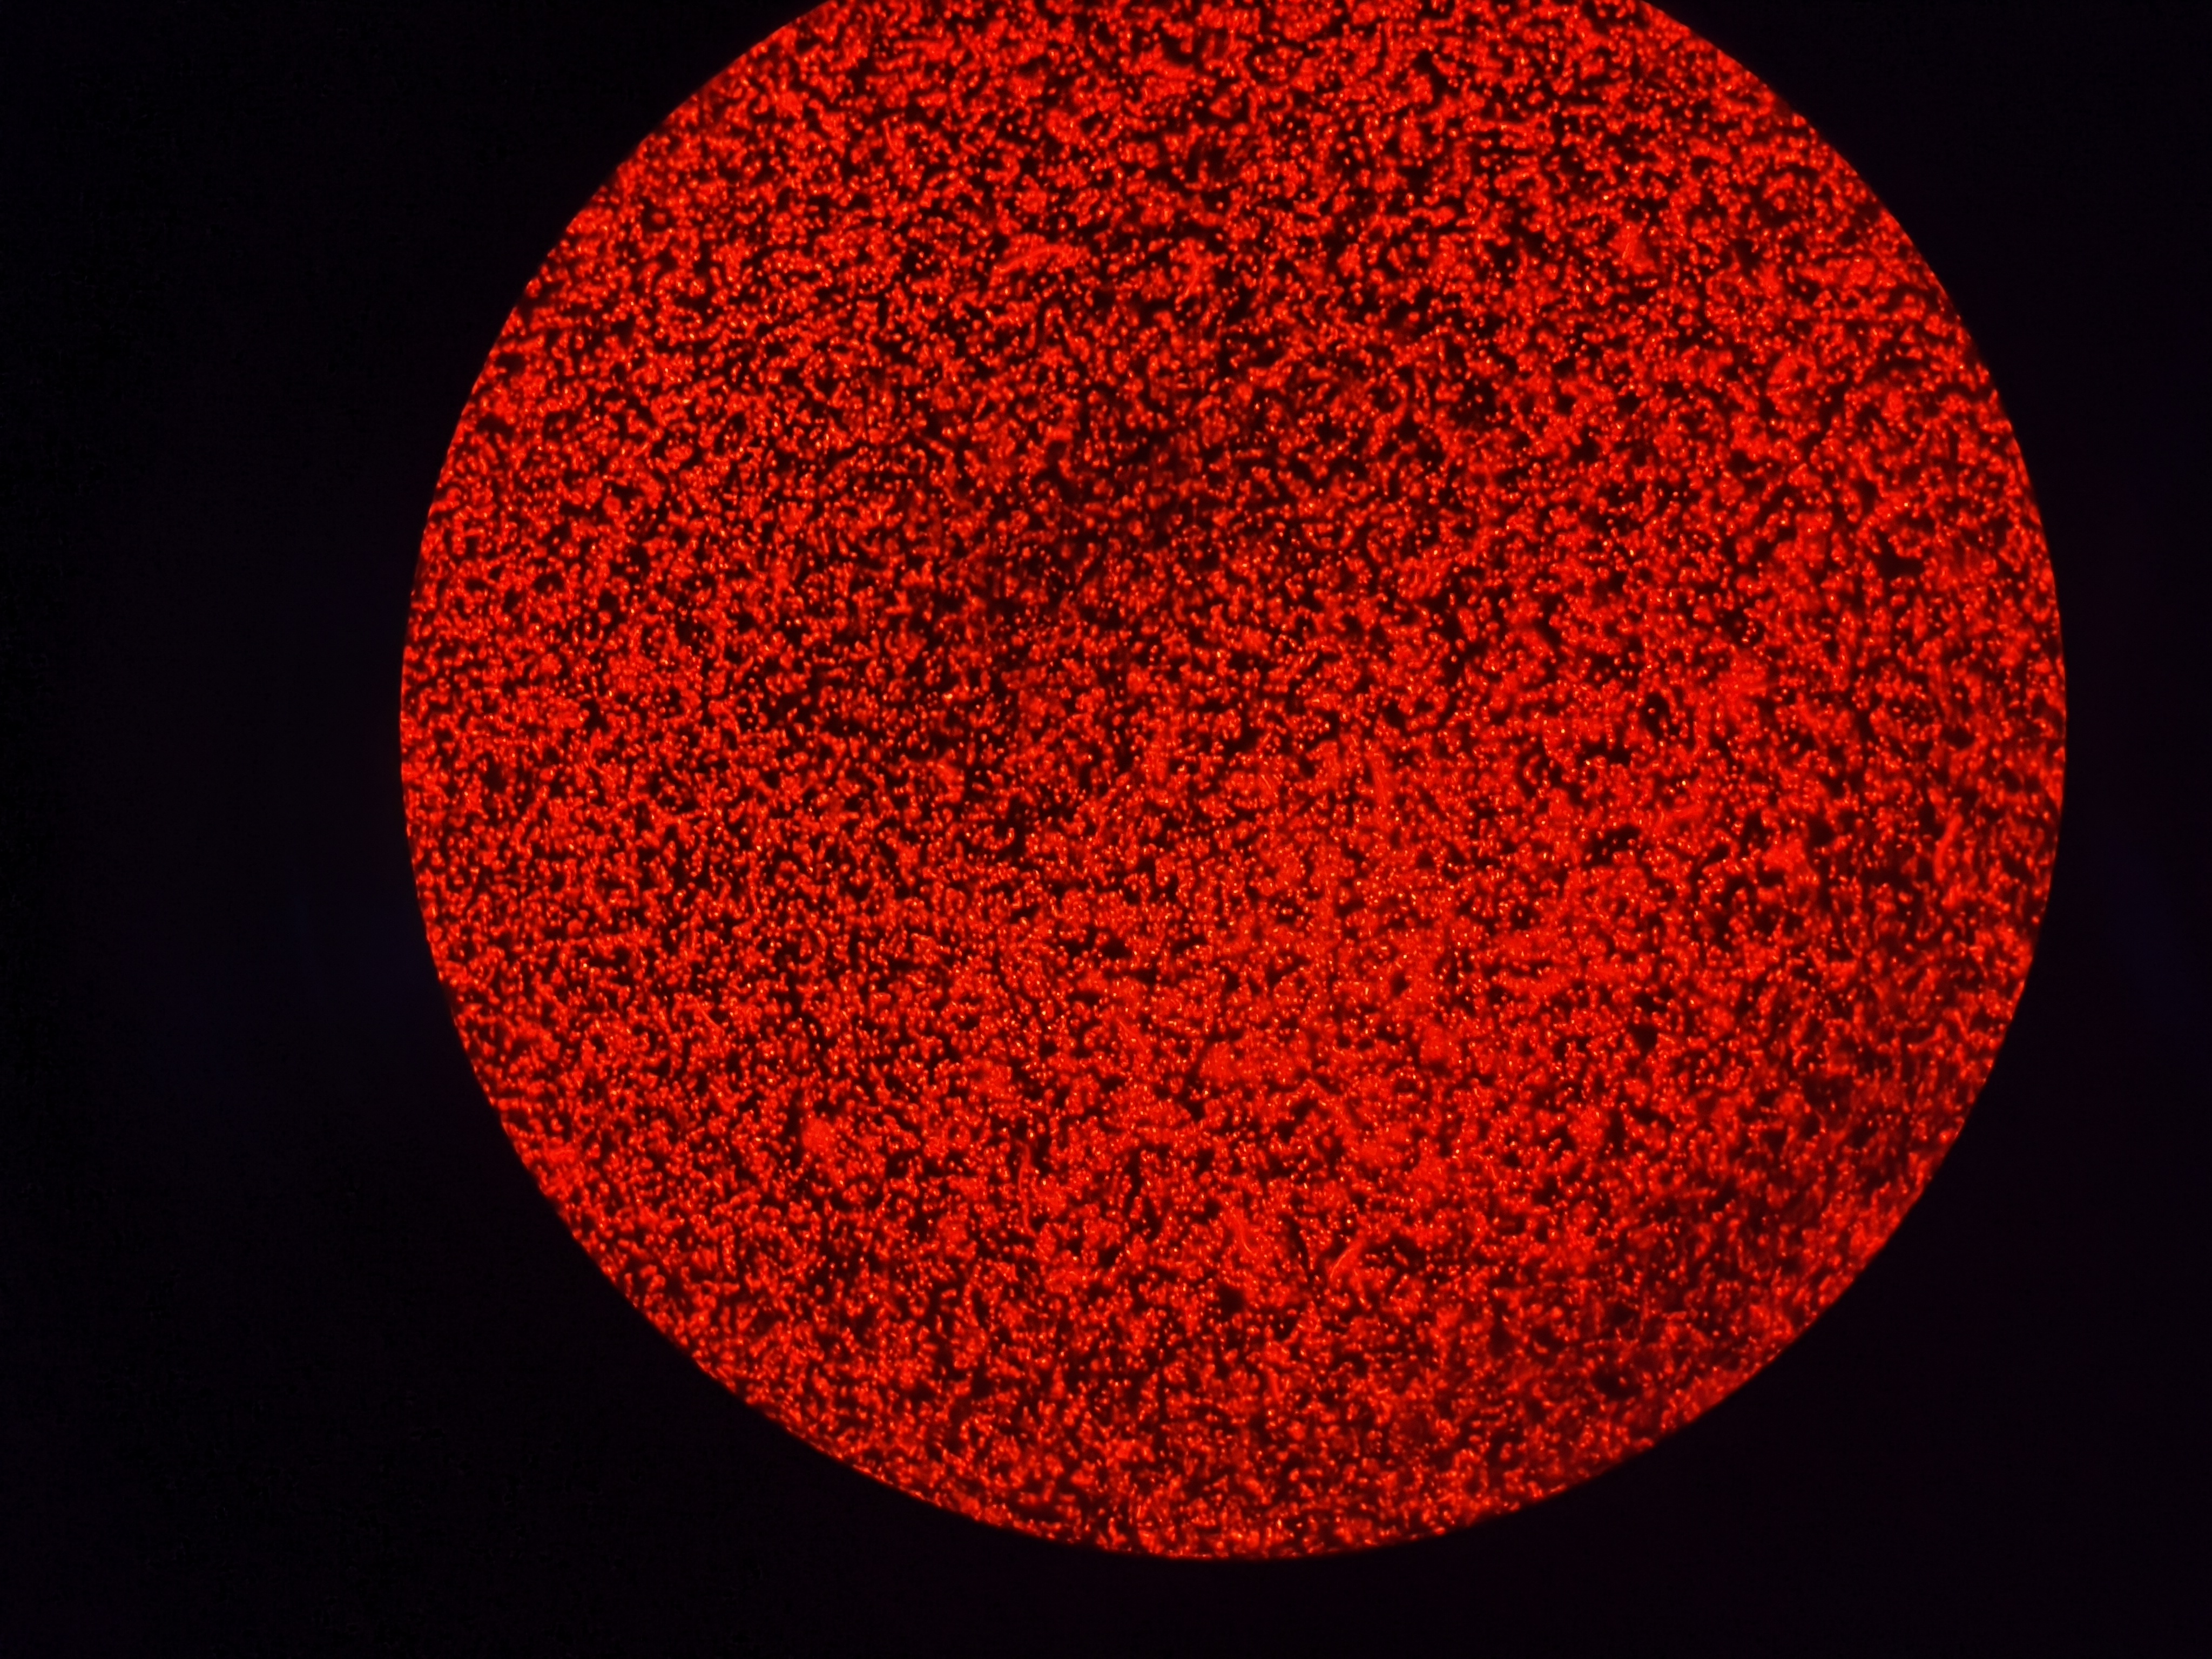
\includegraphics[width=.30\textwidth]{fig/red.jpg}
    \caption{Microscopia de fluorescência de \textit{Escherichia coli}
    transformada com plasmídeo contendo mCherry. Imagem retirada direto da lente
    ocular do microscópio.}
    \label{mCherry}
\end{wrapfigure}
Dentre os três plasmídeos testados, observou-se crescimento
bacteriano positivo em dois casos: (i) as colônias transformadas com o plasmídeo
contendo mCherry exibiram coloração vermelha característica, e (ii) as colônias
transformadas com mTAGbfp2 apresentaram fluorescência azul, conforme evidenciado
pelas imagens de microscopia de fluorescência. Veja a \cref{mCherry} e a
\cref{mTAG}.

\begin{wrapfigure}[11]{r}{0.35\textwidth}
    \centering
    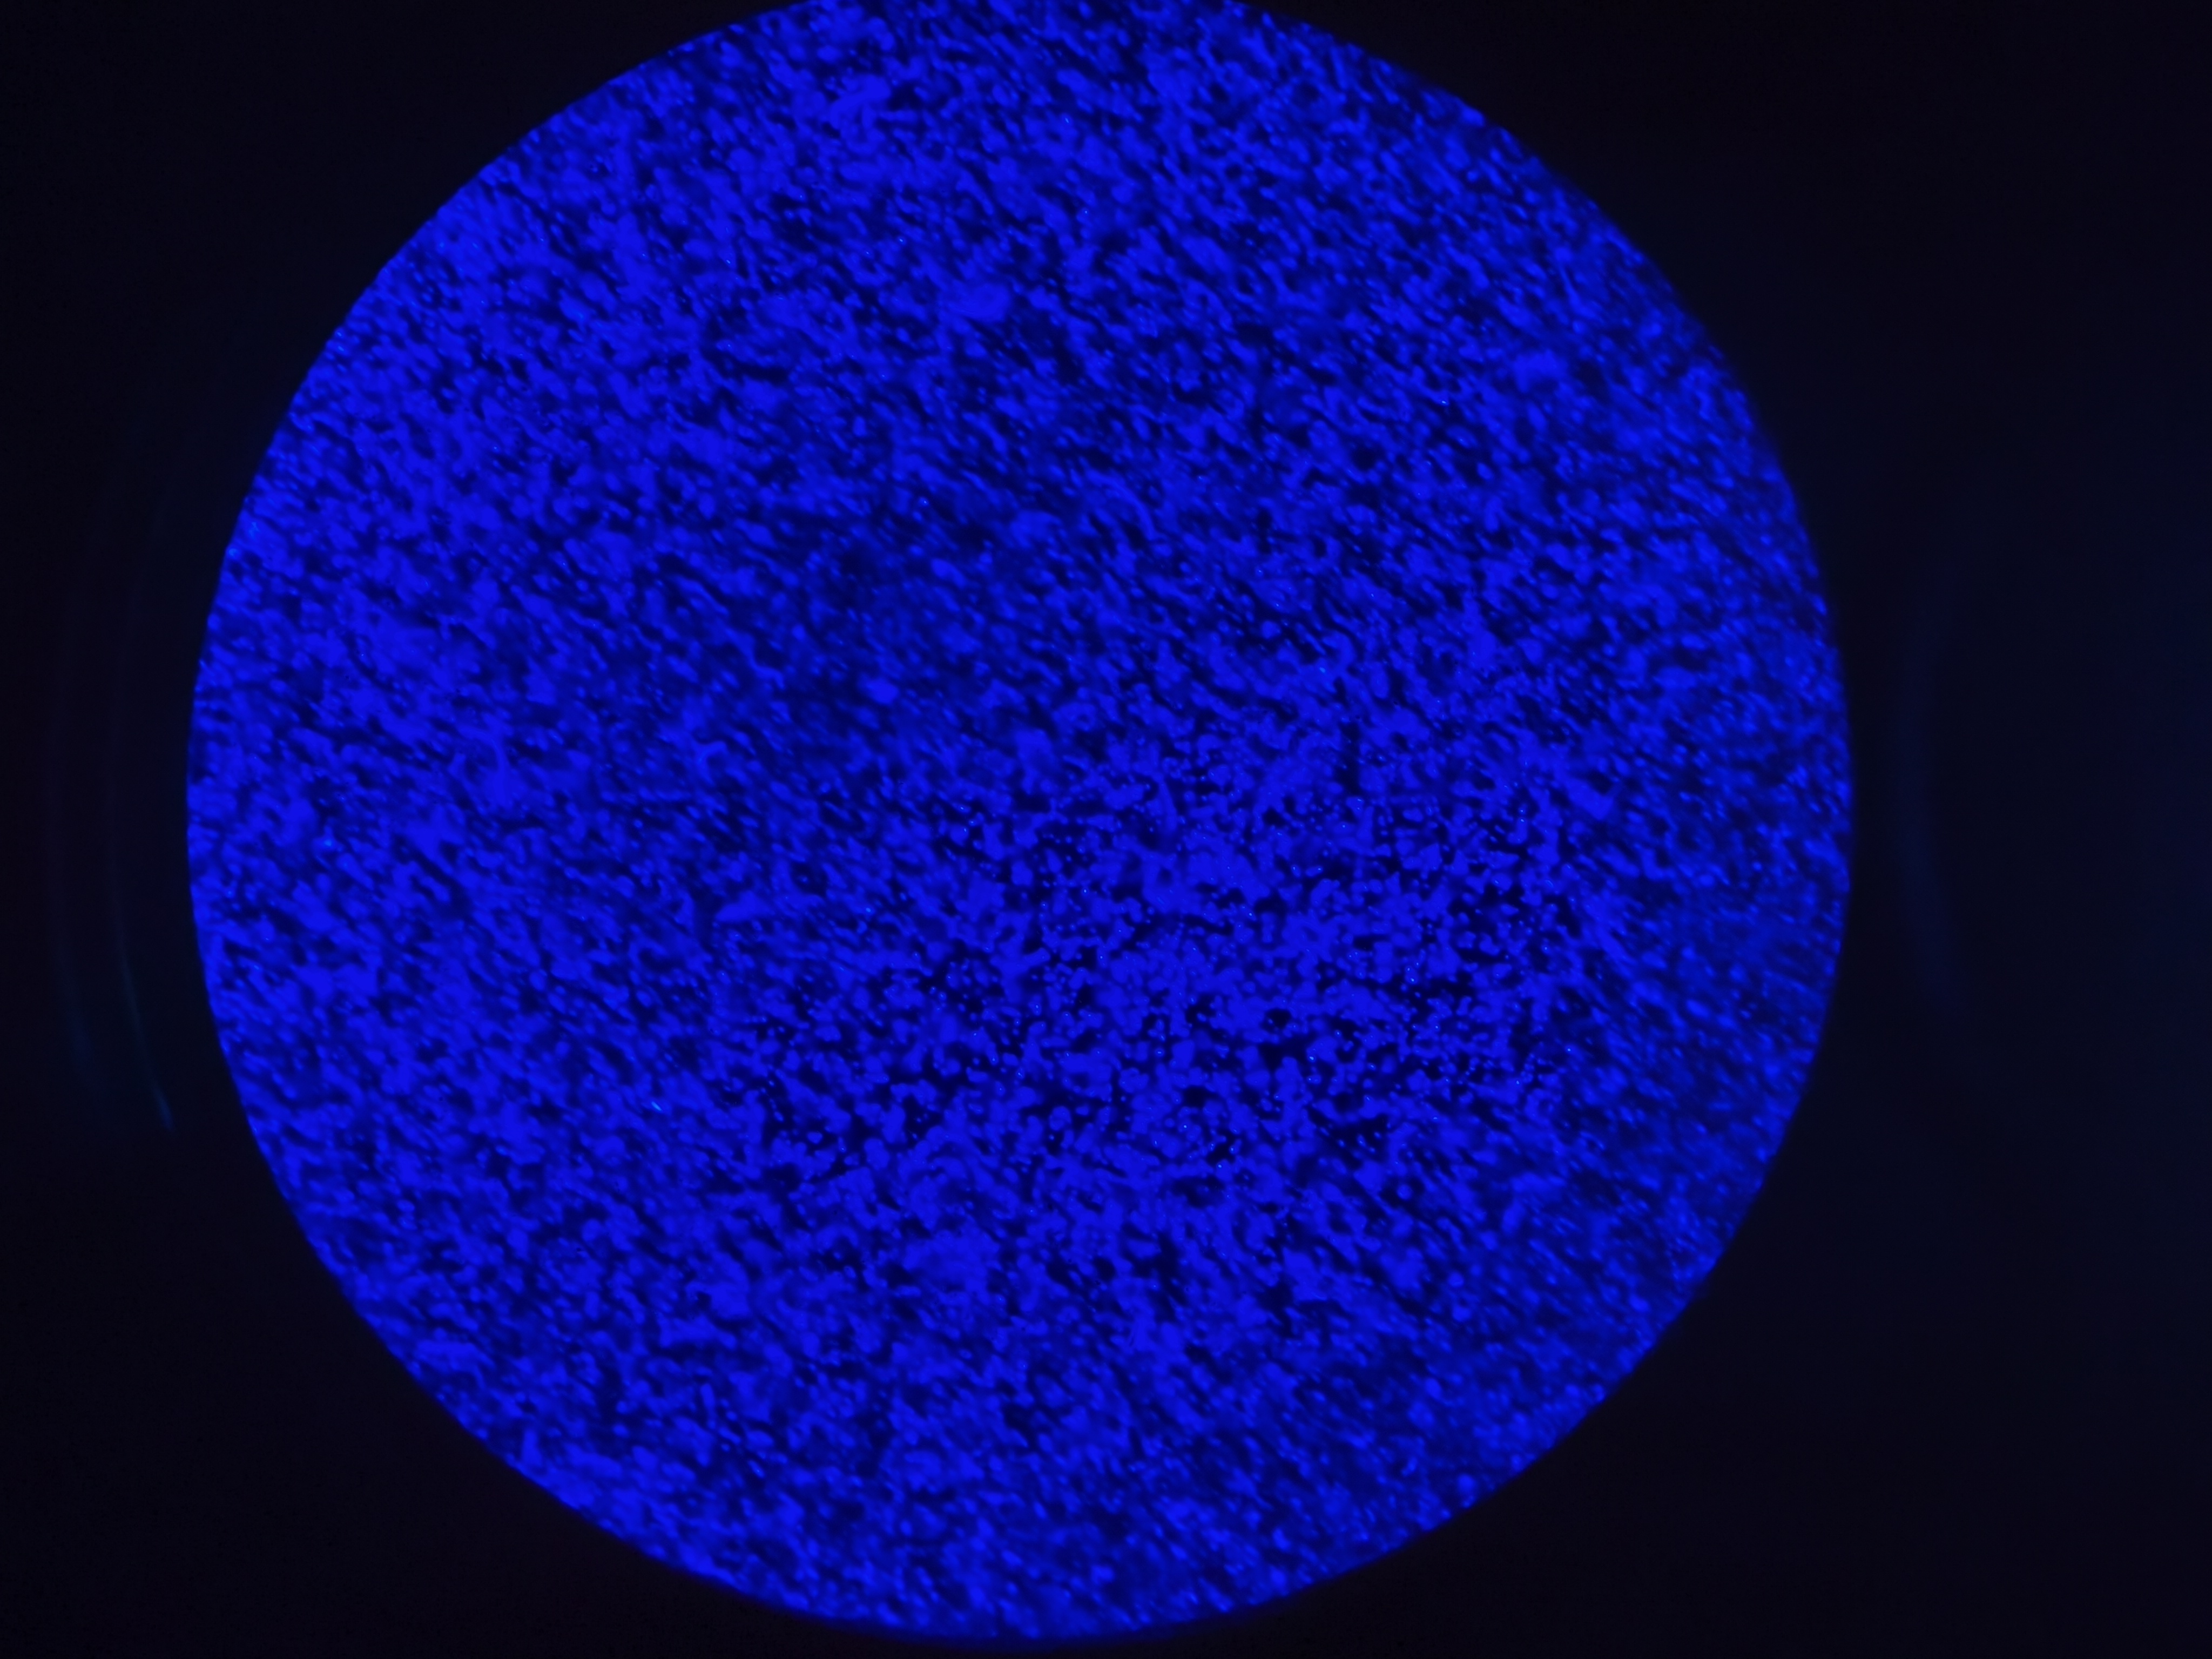
\includegraphics[width=.30\textwidth]{fig/blue.jpg}
    \caption{Microscopia de fluorescência de \textit{Escherichia coli}
    transformada com plasmídeo contendo mTAGbfp2. Imagem retirada direto da lente
    ocular do microscópio.}
    \label{mTAG}
\end{wrapfigure}

Em contraste, a transformação com o plasmídeo contendo GFP não resultou em
colônias viáveis, indicando falha nesse caso específico. Uma análise posterior
revelou que essa falha estava associada à baixa concentração do plasmídeo
durante a transformação, possivelmente devido à quantidade limitada disponível.
Esse fator técnico pode ter comprometido a eficiência da transformação,
explicando a ausência de crescimento bacteriano nessa condição.

Por fim, a correlação entre as cores observadas na transformações bem-sucedidas
e os marcadores genéticos esperados confirma a especificidade dos resultados
obtidos.
